% Lernblatt Terme – Variante „schwach“ – gebaut aus der Aufgabenbank
% (bank/terme) nach Prompt v5.1, Vorbild Muster 4
% (bau/terme/muster-2026-10-01/muster4.tex).
% Blattfolge der Mappe (2026-10-01, sechs Einheiten): 1 Zusammenfassen,
% 2 Malnehmen, 3 Klammern auflösen, 4 Ausklammern, 5 Termwerte,
% 6 Terme aufstellen; Blatt 0 davor, „Zum Schluss“ und Lösungen dahinter.
% „schwach“: feine Leiter (alle Sprossen der Mappe ohne GYM), Vorstufen
% als eigene Nummern vor der Einheit, Grundvorstellung auf Blatt 0.
% Quelle je Teilaufgabe im Kommentar davor: % <id> = aus der Bank,
% % EINGANG <id> = erfundene Aufgabe des Blatts terme-2026-10-01 (neu.jsonl),
% % GEÄNDERT <id> = Form geändert, % NEU = nicht in der Bank.
% % pruef: … = Rechenprobe (pruef.py).
\documentclass[11pt]{article}
\usepackage{mathblatt}
\usepackage{multicol}
\usepackage{lastpage}
% Kopf: nur das Thema; Fuß: „Seite n von m“
\pagestyle{fancy}\fancyhf{}\renewcommand{\headrulewidth}{0pt}
\setlength{\headheight}{14pt}
\fancyhead[L]{\small Terme}
\fancyfoot[C]{\small Seite \thepage\ von \pageref{LastPage}}
\raggedright
\makeatletter
% ---------------------------------------------------------------- Satz
\newcommand{\vorgerechnet}[1]{\textcolor{gray!70}{#1}}
\newcommand{\einheit}[2]{\par\Needspace*{0.33\textheight}\addvspace{16pt}%
  \noindent{\Large\bfseries\ifblank{#1}{}{#1\hspace{0.6em}}#2}\par\nobreak\vspace{2pt}%
  \gappto\mblsg{\lsgeinheit{\ifblank{#1}{}{#1\ }#2}}}
\newsavebox{\nrbox}\newlength{\nrhoehe}
\newcommand{\nrtitel}[1]{\noindent\hangindent1.6em\hangafter1%
  \makebox[1.6em][l]{\textbf{\theaufgabe.}}#1\par\nobreak\vspace{1pt}\nobreak}
\newenvironment{nr}[2][]{\refstepcounter{aufgabe}\setcounter{teil}{0}%
  \def\nrart{#1}%
  \ifx\nrart\@empty
    \begin{lrbox}{\nrbox}\begin{minipage}[t]{\linewidth}\raggedright
    \setlength{\parskip}{0pt}\nrtitel{#2}%
  \else
    \par\addvspace{11pt}\Needspace*{6\baselineskip}\nrtitel{#2}%
  \fi}%
 {\ifx\nrart\@empty
    \end{minipage}\end{lrbox}%
    \setlength{\nrhoehe}{\dimexpr\ht\nrbox+\dp\nrbox\relax}%
    \par\addvspace{11pt}\Needspace*{\nrhoehe}\noindent\usebox{\nrbox}\par
  \else\par\fi}
\newcommand{\teilmarke}{\stepcounter{teil}\makebox[1.6em][r]{\alph{teil})\hspace{0.35em}}}
\newcommand{\marke}[1]{\ifblank{#1}{}{\hfill{\footnotesize #1}}}
\newlength{\feldbreite}\setlength{\feldbreite}{4.5cm}
\newcommand{\antwort}{\underline{\hspace{\feldbreite}}}
\newcommand{\fld}[1][1.2cm]{\underline{\hspace{#1}}}
\newcommand{\zeilenluft}{\par\nobreak\vskip 12pt plus 1pt\relax}
\newcommand{\zeilenluftb}{\par\vskip 12pt plus 1pt\relax}
\newlength{\kw}\newlength{\kwmax}
\newcounter{kzahl}\newcounter{kzeile}
\newcommand{\kliste}{}
\newcommand{\kmerke}[2]{\settowidth{\kw}{#1}%
  \ifdim\kw>\kwmax\global\kwmax=\kw\fi\stepcounter{kzahl}\gappto\kliste{#2}}
\newcommand{\kstart}[1]{\global\kwmax=0pt\setcounter{kzahl}{0}\setcounter{kzeile}{0}%
  \gdef\kliste{}\setlength{\feldbreite}{#1}}
\newcommand{\kende}{\par\nobreak\vspace{3pt}\nobreak\kliste\par}
\newcommand{\kettezeile}[1]{\stepcounter{kzeile}%
  \ifnum\value{kzeile}>1
    \ifnum\value{kzeile}<4 \zeilenluft
    \else\ifnum\numexpr\value{kzahl}-\value{kzeile}\relax<2 \zeilenluft
    \else\zeilenluftb\fi\fi
  \fi
  \noindent#1\par}
\newenvironment{kette}[1][4.5cm]{\kstart{#1}}{\kende}
\newcommand{\termspalte}[1]{\makebox[\kwmax][l]{$#1 =$}\hspace{0.6em}}
\NewDocumentCommand{\rk}{O{} m m}{\kmerke{$#2 =$}{\kettezeile{\teilmarke\lsgm{#3}%
  \termspalte{#2}\antwort\marke{#1}}}}
\newcommand{\rkv}[2]{\kmerke{$#1 =$}{\kettezeile{\teilmarke\termspalte{#1}%
  \vorgerechnet{$#2$}}}}
% Frage in fester Spalte, dann Antwortfeld (Vorstufen): \rfr{Text}{Lösung als Text}
\NewDocumentCommand{\rfr}{O{} m m}{\kmerke{#2}{\kettezeile{\teilmarke\lsgt{#3}%
  \makebox[\kwmax][l]{#2}\hspace{0.6em}\antwort\marke{#1}}}}
\newenvironment{werte}[1][2.8cm]{\kstart{#1}}{\kende}
\newcommand{\wertkopf}[2]{$#1$\hspace{0.8em}für $#2$:}
\NewDocumentCommand{\rw}{O{} m m m}{\kmerke{\wertkopf{#2}{#3}}{\kettezeile{\teilmarke\lsgm{#4}%
  \makebox[\kwmax][l]{\wertkopf{#2}{#3}}\hspace{0.6em}\antwort\marke{#1}}}}
\newcommand{\rwv}[3]{\kmerke{\wertkopf{#1}{#2}}{\kettezeile{\teilmarke
  \makebox[\kwmax][l]{\wertkopf{#1}{#2}}\hspace{0.6em}\vorgerechnet{$#3$}}}}
\NewDocumentCommand{\rt}{O{} m m}{\par\vspace{7pt}\noindent\hangindent1.6em\hangafter1
  \teilmarke\lsgt{#3}#2\nobreak\hspace{0.6em}\underline{\hspace{4cm}}\marke{#1}\par}
% Textzeile ohne Antwortfeld (Felder stehen im Text oder der Schüler markiert im Term)
\NewDocumentCommand{\rto}{O{} m m}{\par\vspace{7pt}\noindent\hangindent1.6em\hangafter1
  \teilmarke\lsgt{#3}#2\marke{#1}\par}
\newlength{\kennbreite}\setlength{\kennbreite}{1.6cm}
\NewDocumentCommand{\rtx}{O{} m m}{\par\vspace{7pt}\noindent
  \ifblank{#1}{\parbox[t]{\linewidth}{\raggedright\hangindent1.6em\hangafter1
   \teilmarke\lsgt{#3}#2}}%
  {\parbox[t]{\dimexpr\linewidth-\kennbreite\relax}{\raggedright\hangindent1.6em\hangafter1
   \teilmarke\lsgt{#3}#2}\parbox[t]{\kennbreite}{\raggedleft\footnotesize #1}}\par}
\NewDocumentCommand{\rs}{O{} m m}{\par\vspace{9pt}\noindent
  \teilmarke\lsgt{#3}%
  \ifblank{#1}{\parbox[t]{\dimexpr\linewidth-1.6em\relax}{\raggedright #2}}%
   {\parbox[t]{\dimexpr\linewidth-1.6em-\kennbreite\relax}{\raggedright #2}%
    \parbox[t]{\kennbreite}{\raggedleft\footnotesize #1}}\par\raum}
\newcommand{\raum}{\par\nobreak\vspace{7mm}\noindent\hspace*{1.6em}%
  \rule{0.5\textwidth}{0.4pt}\par\nobreak\vspace{7mm}\noindent\hspace*{1.6em}%
  \rule{0.5\textwidth}{0.4pt}\par}
\newcommand{\kreuzzeile}[1]{\par\vspace{6pt}\noindent\hspace*{1.6em}#1\par}
\renewcommand{\kreuz}[1]{$\square$\,#1\hspace{2.2em}}
\newcommand{\figurfelder}[2]{\par\vspace{6pt}\noindent\hspace*{1.6em}%
  $\vcenter{\hbox{#1}}$\hspace{1.5em}\begin{tabular}[c]{@{}l@{\hspace{0.5em}}l@{}}#2\end{tabular}\par}
% Merkkasten: schmaler Rahmen, je Zeile ein Fall (Stichwort fett, Beispiel,
% Ergebnis fett), zuletzt „Wichtig:“
\newcommand{\merk}[1]{\par\nobreak\vspace{5pt}\noindent
  \fcolorbox{black!60}{white}{\parbox{\dimexpr\linewidth-2\fboxsep-2\fboxrule\relax}{%
  \raggedright\setlength{\parskip}{1.5pt}#1}}\par\vspace{2pt}}
\newcommand{\mz}[2]{\textbf{#1} #2\par}
% ---------------------------------------------------------------- Lösungen
\newcommand{\mblsg}{}
\newcommand{\lsgm}[1]{\lsgt{$#1$}}
\newcommand{\lsgextra}{}
\newcommand{\lsgt}[1]{\xappto\mblsg{\noexpand\lz{\theaufgabe}{\alph{teil}}}%
  \xappto\mblsg{{\unexpanded{#1}\unexpanded\expandafter{\lsgextra}}}%
  \gdef\lsgextra{}}
\newcommand{\falsch}[1]{\gdef\lsgextra{\quad{\footnotesize falsch $\rightarrow$ Nr.~#1}}}
\newcommand{\falschk}[1]{\gappto\kliste{\falsch{#1}}}
\newcommand{\lzletzte}{0}
\newcommand{\lz}[3]{\par\noindent\hangindent3.4em\hangafter1
  \ifnum#1=\lzletzte\relax\makebox[1.8em][l]{}\else\makebox[1.8em][l]{\textbf{#1}}\fi
  \gdef\lzletzte{#1}%
  \makebox[1.6em][l]{\ifx&#2&\else#2)\fi}#3\par}
\newcommand{\lsgeinheit}[1]{\par\addvspace{4pt}\noindent{\bfseries #1}\par}
\makeatother

\begin{document}
\setlength{\parskip}{0pt}

% =================================================================== Blatt 0
\einheit{}{Das kennst du schon}
\noindent
\begin{minipage}[t]{0.48\linewidth}
\begin{nr}{Plus und Minus}
\begin{kette}[2cm]
% terme-zone-f1-v1
\rk{4 - 9}{-5}
% terme-zone-f1-v4
\rk{-6 - 4}{-10}
% terme-zone-f1-v3
\rk{-2{,}5 + 1}{-1{,}5}
% EINGANG terme-neu-2026-10-01-1
\rk{-3{,}5 - (-6)}{2{,}5}
\end{kette}
\end{nr}
\begin{nr}{Mal mit Vorzeichen}
\begin{kette}[2cm]
% terme-zone-f2-v1
\rk{(-5) \cdot 2}{-10}
% terme-zone-f2-v4
\rk{(-4) \cdot (-5)}{20}
% terme-zone-f2-v3
\rk{(-0{,}5) \cdot 8}{-4}
% EINGANG terme-neu-2026-10-01-2
\rk{(-2{,}5) \cdot (-4)}{10}
\end{kette}
\end{nr}
\end{minipage}\hfill
\begin{minipage}[t]{0.48\linewidth}
\begin{nr}{Dezimalzahlen und Brüche}
\begin{kette}[2cm]
% terme-zone-f3-v4
\rk{0{,}9 + 0{,}3}{1{,}2}
% terme-zone-f3-v3
\rk{0{,}5 - 1{,}5}{-1}
% terme-zone-f3-v2
\rk{\frac{1}{2} + \frac{1}{4}}{\frac{3}{4}}
% EINGANG terme-neu-2026-10-01-3
\rk{-0{,}7 - 0{,}5}{-1{,}2}
\end{kette}
\end{nr}
\begin{nr}{Punkt vor Strich}
\begin{kette}[2cm]
% terme-zone-f4-v1
\rk{5 + 2 \cdot 4}{13}
% terme-zone-f4-v4
\rk{9 - 2 \cdot 3}{3}
% terme-zone-f4-v3
\rk{6 - 4 \cdot 2{,}5}{-4}
% EINGANG terme-neu-2026-10-01-4
\rk{3 - 2 \cdot (-5)}{13}
\end{kette}
\end{nr}
\end{minipage}

\begin{nr}[b]{Was bedeutet die Zahl vor dem $x$? – Schreibe kürzer.}
\begin{kette}[3cm]
% NEU (Grundvorstellung: Vorzahl als Anzahl)
\rk{x + x + x}{3x}
% NEU
\rk{y + y + y + y + 2}{4y + 2}
\end{kette}
% NEU (Grundvorstellung: Term zum Bild ankreuzen)
\rtx{In jedem Kasten liegen $x$ Kugeln. Welcher Term passt zum Bild? Kreuze an.}{$2x + 3$}
\kreuzzeile{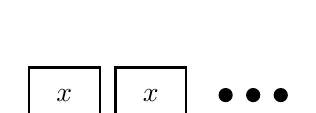
\begin{tikzpicture}[baseline=(current bounding box.center),line width=0.8pt]
\draw (0,0) rectangle (0.9,0.7); \node at (0.45,0.35) {$x$};
\draw (1.1,0) rectangle (2.0,0.7); \node at (1.55,0.35) {$x$};
\fill (2.5,0.35) circle (0.09); \fill (2.85,0.35) circle (0.09); \fill (3.2,0.35) circle (0.09);

\end{tikzpicture}\hspace{2em}\kreuz{$5x$}\kreuz{$2x + 3$}\kreuz{$x + 5$}}
\end{nr}

% =================================================================== Einheit 1
\einheit{1}{Terme zusammenfassen}
\merk{\mz{Gleiche Variablen:}{Vorzahlen addieren, die Variable bleibt: $3x + 5x = \mathbf{8x}$}
\mz{Zahl ohne Variable bleibt:}{$7a - 2a + 4 = \mathbf{5a + 4}$}
\mz{Hochzahl zählt mit:}{$x^2 + 3x$ \textbf{bleibt so}}
\mz{Wichtig:}{$3x + 4$ ist nicht $7x$. $x$ hat die Vorzahl 1: $x + 6x = 7x$, nicht $6x$.}}

\begin{nr}[b]{Unterstreiche, was zusammengehört.}
% terme-e2-k1-s0-v1
\rto{$4y$,\quad $7$,\quad $9y$}{$4y$ und $9y$}
% terme-e2-k1-s0-v2
\rto{$6$,\quad $2a$,\quad $8$,\quad $a$}{$2a$ und $a$; $6$ und $8$}
% terme-e2-k1-s0-v4
\rto{$7b$,\quad $2c$,\quad $5b$,\quad $4$}{$7b$ und $5b$}
% terme-e2-k1-s0-v3
\rto{$5x^2$,\quad $4x$,\quad $3x^2$}{$5x^2$ und $3x^2$}
% NEU (Produkt zweier Variablen ist eine eigene Sorte)
\rto{$3ab$,\quad $2a$,\quad $5b$,\quad $ab$}{$3ab$ und $ab$}
% NEU (zwei Variablen mit Potenz: $xy^2$ und $x^2y$ sind verschieden)
\rto{$2xy^2$,\quad $3x^2y$,\quad $4xy^2$,\quad $x^2y$}{$2xy^2$ und $4xy^2$; $3x^2y$ und $x^2y$}
\end{nr}

\noindent
\begin{minipage}[t]{0.40\linewidth}
\begin{nr}{Welche Vorzahl hat die Variable?}
\begin{kette}[2.5cm]
% terme-e2-k2-s0-v1
\rfr{$a$}{$1$ (denn $a = 1a$)}
% terme-e2-k2-s0-v2
\rfr{$-b$}{$-1$ (denn $-b = -1b$)}
% terme-e2-k2-s0-v3
\rfr{$1{,}5z$}{$1{,}5$}
% terme-e2-k2-s0-v4
\rfr{$-4w$}{$-4$}
\end{kette}
\end{nr}

\end{minipage}\hfill
\begin{minipage}[t]{0.56\linewidth}
\begin{nr}{Schreibe die Glieder mit ihrem Vorzeichen auf.}
\begin{kette}[4cm]
% terme-e2-k3-s0-v1
\rfr{$5a - 2b + 7$}{$+5a$, $-2b$, $+7$}
% terme-e2-k3-s0-v2
\rfr{$-3x + 6 - y$}{$-3x$, $+6$, $-y$}
% terme-e2-k3-s0-v3
\rfr{$2m - 9 - 5k$}{$+2m$, $-9$, $-5k$}
% terme-e2-k3-s0-v4
\rfr{$-6 + 3c - 4d$}{$-6$, $+3c$, $-4d$}
\end{kette}
\end{nr}
\end{minipage}

\begin{nr}[b]{Fasse zusammen.}\label{nr:zus}
\begin{kette}
% terme-e2-k4-s1-v1
\rk{7x + 2x}{9x}
% terme-e2-k4-s1-v4
\rk{7x + 8x}{15x}
% terme-e2-k4-s2-v1
\rk{9x - 4x}{5x}
% terme-e2-k4-s3-v1
\rk{2x + 4x + 3x}{9x}
% terme-e2-k4-s4-v1
\rk{5x + 3 + 2x}{7x + 3}
% terme-e2-k4-s5-v2
\rk{2x + 5y + 4x}{6x + 5y}
% terme-e2-k4-s6-v1
\rk{y + 4y}{5y}
% terme-e2-k4-s7-v1
\rk{2x - 7x}{-5x}
\end{kette}
\end{nr}

\begin{nr}[b]{Fasse zusammen – achte auf Vorzeichen und Hochzahlen.}\label{nr:zusb}
\begin{kette}
% terme-e2-k4-s8-v2
\rk{-5a + 9a}{4a}
% NEU (negatives erstes Glied, Vorzahl 1 und zwei Zahlglieder)
\rk{-a + 7 + 3a - 2}{2a + 5}
% terme-e2-k4-s9-v1
\rk{4x^2 + 5x + 2x^2}{6x^2 + 5x}
% terme-e2-k4-s10-v2
\rk{4{,}2a - 1{,}2a}{3a}
% NEU (Potenz und Dezimalvorzahl, negatives Ergebnis)
\rk{0{,}5y^2 + 3y - 2y^2}{-1{,}5y^2 + 3y}
\end{kette}
% terme-e2-k6-s4-v2
% pruef: s + 2*s + s + 2*s == 6*s
% pruef: 6*8 == 48
\rs{Ein Beet ist $s$ Meter breit und doppelt so lang. Um das Beet kommt ein Zaun. Stelle einen Term für die Länge des Zauns auf und fasse ihn zusammen. Wie viele Meter Zaun braucht man bei $s = 8$?}{$s + 2s + s + 2s = 6s$; für $s = 8$: $48$ m}
% terme-e2-k4-s11-v1
% pruef: 8*a - 2*a**2 - 5*a == 3*a - 2*a**2
% pruef: 3*3 - 2*3**2 == -9
\rs[P10 ’25]{Vereinfache den Term $8a - 2a^2 - 5a$ und berechne seinen Wert für $a = 3$.}{$3a - 2a^2$; für $a = 3$: $-9$}
\end{nr}

% =================================================================== Einheit 2
\einheit{2}{Terme malnehmen}
\merk{\mz{Zahl mal Term:}{$3 \cdot 4x = \mathbf{12x}$}
\mz{Term mal Term:}{Zahlen mal Zahlen, Variablen mal Variablen: $2x \cdot 3x = \mathbf{6x^2}$}
\mz{Zwei Variablen:}{$3a \cdot 2b = \mathbf{6ab}$}
\mz{Wichtig:}{$x \cdot x$ ist $x^2$, nicht $2x$. Minus mal Minus gibt Plus.}}

\begin{nr}[b]{Multipliziere.}\label{nr:mal}
\begin{kette}
% terme-e2-k5-s1-v1
\rk{5 \cdot 2x}{10x}
% terme-e2-k5-s1-v3
\rk{5 \cdot 6x}{30x}
% terme-e2-k5-s2-v2
\rk{7b \cdot 4}{28b}
% terme-e2-k5-s3-v1
\rk{4y \cdot 2y}{8y^2}
% terme-e2-k5-s4-v2
\rk{3 \cdot (-6a)}{-18a}
% terme-e2-k5-s5-v2
\rk{2x \cdot 7y}{14xy}
% terme-e2-k5-s6-v1
\rk{2 \cdot 5x \cdot 3}{30x}
% terme-e2-k5-s7-v3
\rk{3y \cdot (-5x)}{-15xy}
\end{kette}
\end{nr}

\begin{nr}[b]{Multipliziere – mit Potenz und Bruch.}
\begin{kette}
% NEU (drei Faktoren, zwei negativ, Potenz entsteht)
\rk{(-2a) \cdot 3a \cdot (-a)}{6a^3}
% NEU (Bruch als Vorzahl, zwei Variablen)
\rk{\frac{1}{2}x \cdot 6y}{3xy}
\end{kette}
% NEU (Abschluss Anwendung: Volumen und Kantensumme eines Quaders)
% pruef: a*2*a*3 == 6*a**2
% pruef: 4*(a + 2*a + 3) == 12*a + 12
\rs{Ein Quader ist $a$ cm lang, $2a$ cm breit und 3 cm hoch. Schreibe einen Term für das Volumen in cm³. Schreibe dann einen Term für die Länge aller 12 Kanten zusammen und fasse ihn zusammen.}{Volumen $a \cdot 2a \cdot 3 = 6a^2$; Kanten $4 \cdot (a + 2a + 3) = 12a + 12$}
\end{nr}

% =================================================================== Einheit 3
\einheit{3}{Klammern auflösen}
\merk{\mz{Plus vor der Klammer:}{Klammer weglassen: $a + (b - c) = \mathbf{a + b - c}$}
\mz{Minus vor der Klammer:}{alle Vorzeichen drehen: $a - (b - c) = \mathbf{a - b + c}$}
\mz{Zahl mal Klammer:}{jedes Glied malnehmen: $3 \cdot (x + 4) = \mathbf{3x + 12}$}
\mz{Wichtig:}{Bei der Minusklammer dreht sich jedes Vorzeichen in der Klammer, nicht nur das erste.}}

\begin{nr}[b]{Was steht direkt vor der Klammer: Plus, Minus oder eine Zahl?}
\begin{kette}[3cm]
% terme-e3-k1-s0-v1
\rfr{$7 + (a - 2)$}{ein Plus}
% terme-e3-k1-s0-v2
\rfr{$10 - (b + 4)$}{ein Minus}
% terme-e3-k1-s0-v3
\rfr{$5 \cdot (x - 1)$}{die Zahl $5$ als Faktor}
% terme-e3-k1-s0-v4
\rfr{$2y - 6 \cdot (y + 1)$}{$-6$ als Faktor}
\end{kette}
\end{nr}

\begin{nr}[b]{Plusklammer und Minusklammer – löse auf.}\label{nr:pm}
\begin{kette}
% terme-e3-k2-s1-v1 (vorgerechnet)
\rkv{5a + (2b - 1)}{5a + 2b - 1}
% terme-e3-k2-s1-v3
\rk{5a + (2b - 4)}{5a + 2b - 4}
\end{kette}
% terme-e3-k2-s3-v1
% pruef: 30 - (12 + 8) == 10
% pruef: 30 - 12 - 8 == 10
\rs{Rechne $30 - (12 + 8)$ auf zwei Wegen: erst die Klammer ausrechnen und dann abziehen; dann Glied für Glied abziehen. Vergleiche beide Ergebnisse.}{$30 - 20 = 10$ und $30 - 12 - 8 = 10$; beide Wege ergeben 10}
\begin{kette}
% terme-e3-k2-s4-v1
\rk{5a - (2b + 4)}{5a - 2b - 4}
% terme-e3-k2-s5-v1
\rk{7a - (2b - 5 + c)}{7a - 2b + 5 - c}
% EINGANG terme-neu-2026-10-01-9
\rk{2{,}5 - (-a + 1{,}5b - 3{,}5)}{a - 1{,}5b + 6}
% NEU (drei Klammern mit Potenzen, auflösen und zusammenfassen)
\rk{(x^2 + 2x) - (3x - 4) + (x^2 - 1)}{2x^2 - x + 3}
\end{kette}
\end{nr}

\begin{nr}[b]{Mal Klammer – löse die Klammer auf.}\label{nr:mk}
\begin{kette}
% GEÄNDERT terme-e3-k2-s2-v1 (Form: ohne Tabelle; vorgerechnet)
\rkv{5 \cdot (x + 3)}{5 \cdot x + 5 \cdot 3 = 5x + 15}
% GEÄNDERT terme-e3-k2-s2-v2 (Form: ohne Tabelle)
\rk{4 \cdot (a + 7)}{4a + 28}
% terme-e3-k2-s6-v2
\rk{-3 \cdot (a - 7)}{-3a + 21}
% NEU (Variable mal Klammer, Potenz entsteht)
\rk{2x \cdot (x + 5)}{2x^2 + 10x}
% NEU (negative Zahl hinter der Klammer, drei Glieder)
\rk{(a - 2b + 3) \cdot (-4)}{-4a + 8b - 12}
% NEU (Dezimalfaktor mit Variable, drei Glieder)
\rk{0{,}5a \cdot (4a - 6 + 2b)}{2a^2 - 3a + ab}
\end{kette}
\end{nr}

\begin{nr}[b]{Löse die Klammern auf und fasse zusammen.}\label{nr:kz}
\begin{kette}
% terme-e3-k2-s7-v1 (vorgerechnet)
\rkv{5x + 2 \cdot (x + 6)}{5x + 2x + 12 = 7x + 12}
% terme-e3-k2-s7-v2
\rk{9a - (4a + 3)}{5a - 3}
% terme-e3-k2-s8-v1
\rk{3 \cdot (2x + 5) - 2 \cdot (x - 4)}{4x + 23}
% NEU (zwei Klammern mit Variable davor)
\rk{2x \cdot (x + 3) - x \cdot (x - 1)}{x^2 + 7x}
% NEU (Klammer in der Klammer)
\rk{5a - [\,2 - (a + 3)\,]}{6a + 1}
\end{kette}
% terme-e3-k3-s4-v3
% pruef: 2.5*(20 + x) == 50 + 2.5*x
% pruef: 50 + 2.5*4 == 60
\rs{Ein Muffin kostet 2,50 €. Für eine Feier werden 20 Muffins bestellt und noch $x$ Muffins dazu. Schreibe den Preis in Euro als Term mit Klammer. Löse die Klammer auf. Was kosten die Muffins bei $x = 4$?}{$2{,}50 \cdot (20 + x) = 50 + 2{,}50x$; für $x = 4$: $60\,€$}
\end{nr}

\begin{nr}{Abschluss}
\begin{kette}
% NEU
\rk{4 \cdot (y - 2) - (y - 5)}{3y - 3}
\end{kette}
% GEÄNDERT terme-e3-k3-s3-v2 (Form: Feld neben der Tabelle)
% pruef: 2*(a + 6) == 2*a + 12
\rtx{Die Tabelle zeigt eine aufgelöste Klammer. Welcher Term mit Klammer gehört dazu?}{$2 \cdot (a + 6) = 2a + 12$}
\figurfelder{\sachtabelle{ccc}{$\cdot$ & $a$ & $+6$}{$2$ & $2a$ & $+12$}}{Term mit Klammer: & \underline{\hspace{4cm}}}
% terme-e3-k3-s2-v2
% pruef: 15 - (x - 3) == 18 - x
\rs{Kai sagt: „Bei $15 - (x - 3)$ muss ich nur das Vorzeichen von $x$ umdrehen. Das ergibt $15 - x - 3$.“ Stimmt das? Begründe.}{Nein: Minus vor der Klammer dreht jedes Vorzeichen, $15 - x + 3 = 18 - x$}
\end{nr}

% =================================================================== Einheit 4
\einheit{4}{Ausklammern}
\merk{\mz{Zahl ausklammern:}{$6x + 9 = \mathbf{3 \cdot (2x + 3)}$}
\mz{Variable ausklammern:}{$4a^2 + 2a = \mathbf{2a \cdot (2a + 1)}$}
\mz{Probe:}{ausmultiplizieren, es muss der Anfangsterm herauskommen: $2a \cdot 2a + 2a \cdot 1 = \mathbf{4a^2 + 2a}$}
\mz{Wichtig:}{Ist ein Glied selbst der Faktor, bleibt in der Klammer eine 1: $8x - 8 = 8 \cdot (x - 1)$, nicht $8 \cdot x$.}}

\begin{nr}[b]{Welcher Faktor steckt in jedem Glied? Schreibe ihn auf, klammere noch nichts aus.}
\begin{kette}[3cm]
% terme-e4-k1-s0-v1
\rfr{$8x + 12$}{die Zahl $4$}
% terme-e4-k1-s0-v2
\rfr{$9y^2 + 2y$}{die Variable $y$}
% terme-e4-k1-s0-v3
\rfr{$6a^2 + 10a$}{$2a$ (Zahl und Variable)}
% terme-e4-k1-s0-v4
\rfr{$9x - 6 + 15x^2$}{die Zahl $3$}
\end{kette}
\end{nr}

\begin{nr}[b]{Schreibe jedes Glied als Produkt mit dem Faktor.}
% terme-e4-k2-s-1-v1
\rto{$8x + 20 = 4 \cdot$ \fld $\;+\; 4 \cdot$ \fld}{$2x$ und $5$}
% terme-e4-k2-s-1-v2
\rto{$6a + 14 = 2 \cdot$ \fld $\;+\; 2 \cdot$ \fld}{$3a$ und $7$}
% terme-e4-k2-s-1-v3
\rto{$10y + 15 = 5 \cdot$ \fld $\;+\; 5 \cdot$ \fld}{$2y$ und $3$}
\end{nr}

\begin{nr}[b]{Der Faktor steht schon vor der Klammer. Fülle die Klammer.}
% terme-e4-k2-s0-v1
\rto{$9x + 21 = 3 \cdot ($\fld $\;+\;$ \fld$)$}{$3x$ und $7$}
% terme-e4-k2-s0-v2
\rto{$4y + 10 = 2 \cdot ($\fld $\;+\;$ \fld$)$}{$2y$ und $5$}
% terme-e4-k2-s0-v4
\rto{$14b + 21 = 7 \cdot ($\fld $\;+\;$ \fld$)$}{$2b$ und $3$}
\end{nr}

\begin{nr}[b]{Klammere den größten gemeinsamen Faktor aus.}\label{nr:aus}
\begin{kette}
% terme-e4-k2-s1-v1
\rk{5x + 10}{5 \cdot (x + 2)}
% terme-e4-k2-s1-v5
\rk{5x + 40}{5 \cdot (x + 8)}
% terme-e4-k2-s2-v1
\rk{x^2 + 5x}{x \cdot (x + 5)}
% terme-e4-k2-s3-v2
\rk{8a^2 - 20a}{4a \cdot (2a - 5)}
% terme-e4-k2-s4-v1
\rk{6x + 6}{6 \cdot (x + 1)}
% terme-e4-k2-s5-v1
\rk{3x^2 + 6x + 15}{3 \cdot (x^2 + 2x + 5)}
% NEU (negativer Faktor mit zwei Variablen, drei Glieder)
\rk{-4xy - 8y + 2y^2}{-2y \cdot (2x + 4 - y)}
% NEU (Dezimalfaktor mit Variable, Eins bleibt in der Klammer)
\rk{0{,}5a^2 + 0{,}5a}{0{,}5a \cdot (a + 1)}
\end{kette}
\end{nr}

\begin{nr}[b]{Klammere aus und schreibe die Probe (ausmultiplizieren) dahinter.}\label{nr:probe}
\begin{kette}[7.5cm]
% terme-e4-k2-s6-v1
\rk{6x + 30}{6 \cdot (x + 5) = 6x + 30}
% terme-e4-k2-s6-v2
\rk{4a^2 + 20a}{4a \cdot (a + 5) = 4a^2 + 20a}
% terme-e4-k2-s10-v2
\rk{5x^2 + 10xy - 15x}{5x \cdot (x + 2y - 3) = 5x^2 + 10xy - 15x}
\end{kette}
\end{nr}

\begin{nr}{Abschluss}
\begin{kette}
% EINGANG terme-neu-2026-10-01-20
\rk{12ab - 18b}{6b \cdot (2a - 3)}
\end{kette}
% GEÄNDERT terme-e4-k2-s7-v1 (Form: Figur mit Feldern)
% pruef: 4*x + 4*6 == 4*(x + 6)
\rtx{Zwei Rechtecke liegen nebeneinander (Maße in cm). Gib den Flächeninhalt der ganzen Figur als Summe der Teilflächen und als Produkt mit Klammer an.}{Summe: $4x + 24$; Produkt: $4 \cdot (x + 6)$}
\figurfelder{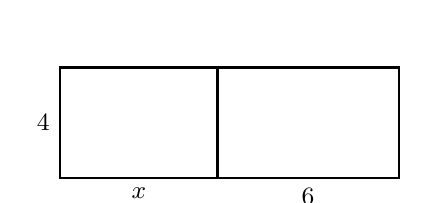
\begin{tikzpicture}[line width=0.8pt]
\draw (0,0) rectangle (2.0,1.4); \draw (2.0,0) rectangle (4.3,1.4);
\node[left,font=\small] at (0,0.7) {$4$};
\node[below,font=\small] at (1.0,0) {$x$};
\node[below,font=\small] at (3.15,0) {$6$};
\end{tikzpicture}}{Summe: & \underline{\hspace{4cm}} \\[8mm]
Produkt: & \underline{\hspace{4cm}}}
% terme-e4-k2-s8-v1
% pruef: 0.1*40 + 0.1*25 == 0.1*(40 + 25)
% pruef: 0.1*65 == 6.5
\rs{Eine Hose kostet 40 €, ein Hemd 25 €. Es gibt 10 \% Rabatt. Anna rechnet den Rabatt mit $0{,}1 \cdot 40 + 0{,}1 \cdot 25$, Ben mit $0{,}1 \cdot (40 + 25)$. Ergeben beide Terme denselben Rabatt? Begründe und berechne den Rabatt.}{Ja, $0{,}1$ ist ausgeklammert; Rabatt $0{,}1 \cdot 65 = 6{,}50\,€$}
\end{nr}

% =================================================================== Einheit 5
\einheit{5}{Termwerte berechnen}
\merk{\mz{Einsetzen:}{$4x - 1$ für $x = 3$: $4 \cdot 3 - 1 = \mathbf{11}$ (Punkt vor Strich)}
\mz{Negative Zahl:}{in Klammern einsetzen: $3x^2$ für $x = -2$: $3 \cdot (-2)^2 = \mathbf{12}$}
\mz{Wichtig:}{$(-2)^2 = 4$, nicht $-4$. Die Klammer beim Einsetzen nicht weglassen.}}

\begin{nr}[b]{Berechne den Wert des Terms.}\label{nr:wert}
\begin{werte}
% terme-e1-k2-s1-v1 (vorgerechnet)
\rwv{4x - 3}{x = 5}{4 \cdot 5 - 3 = 17}
% terme-e1-k2-s1-v2
\rw{2x + 9}{x = -3}{3}
% terme-e1-k2-s1-v3
\rw{10 - 3x}{x = -2}{16}
% NEU (Quadrat bei negativer Einsetzung)
\rw{x^2 + 3x}{x = -4}{4}
% NEU (negativer Bruch als Einsetzung beim Quadrat)
\rw{4x^2}{x = -\frac{1}{2}}{1}
% NEU (zwei Variablen, Bruch als Vorzahl und als Einsetzung)
\rw{\frac{1}{2}a + 3b}{a = 6,\ b = -\frac{1}{2}}{1{,}5}
% NEU (Quadrat einer Klammer, zwei Variablen)
\rw{(x - y)^2 + 2x}{x = 3,\ y = 5}{10}
\end{werte}
\end{nr}

% =================================================================== Einheit 6
\einheit{6}{Terme aufstellen}
\merk{\mz{Vermindert um:}{„$x$ um 5 vermindert“: $\mathbf{x - 5}$}
\mz{Das Mehrfache einer Summe:}{„das Dreifache der Summe aus $x$ und 4“: $\mathbf{3 \cdot (x + 4)}$, mit Klammer}
\mz{Figur:}{Umfang Rechteck mit Seiten $x$ und 3: $x + 3 + x + 3 = \mathbf{2x + 6}$}
\mz{Wichtig:}{„5 vermindert um $x$“ ist $5 - x$, nicht $x - 5$. Ohne Klammer wird nur das erste Glied vervielfacht.}}

\begin{nr}[b]{Kreuze den Term an, der passt.}\label{nr:kreuz}
% terme-e1-k1-s1-v1
\rtx{Das Vierfache einer Zahl $x$ wird um 3 vermindert.}{$4x - 3$}
\kreuzzeile{\kreuz{$4x - 3$}\kreuz{$4 \cdot (x - 3)$}\kreuz{$3 - 4x$}}
% terme-e1-k1-s1-v3
\rtx{Das Vierfache einer Zahl $x$ wird um 6 vermindert.}{$4x - 6$}
\kreuzzeile{\kreuz{$4 \cdot (x - 6)$}\kreuz{$6 - 4x$}\kreuz{$4x - 6$}}
% NEU (Grundfall mit „vergrößert“)
\rtx{Das Doppelte einer Zahl $x$ wird um 4 vergrößert.}{$2x + 4$}
\kreuzzeile{\kreuz{$2 \cdot (x + 4)$}\kreuz{$2x + 4$}\kreuz{$4x + 2$}}
% terme-e1-k1-s7-v4
\rtx[P10 ’17]{Das Doppelte einer Zahl $x$ wird um neun vermindert.}{$2x - 9$}
\kreuzzeile{\kreuz{$2 \cdot (x - 9)$}\kreuz{$9 - 2x$}\kreuz{$2x - 9$}\kreuz{$2x - 9x$}}
% terme-e1-k1-s7-v1
\rtx[P10 ’23]{Die Differenz aus dem Dreifachen einer Zahl $x$ und 7 wird verdoppelt.}{$2 \cdot (3x - 7)$}
\kreuzzeile{\kreuz{$(3x - 7) : 2$}\kreuz{$3x : 7 \cdot 2$}\kreuz{$2 \cdot (3x - 7)$}\kreuz{$3x - 7 \cdot 2$}}
\end{nr}

\begin{nr}[b]{Schreibe einen Term.}\label{nr:auf}
% terme-e1-k1-s2-v2
% pruef: 2*x - 5 == 2*x - 5
\rt{Das Doppelte einer Zahl $x$ wird um 5 vermindert.}{$2x - 5$}
% GEÄNDERT terme-e1-k1-s3-v3 (Form: Feld neben der Figur)
% pruef: 7 + x + 7 + x == 2*x + 14
\rtx{Umfang des Rechtecks (Maße in cm):}{$7 + x + 7 + x = 2x + 14$}
\figurfelder{\rechteck[seiten={7,x,,},punkte=]{3.2}{1.1}}{& \underline{\hspace{4cm}}}
% terme-e1-k1-s4-v1
% pruef: 4*a + 3*b == 4*a + 3*b
\rt{Ein Heft kostet $a$ Euro, ein Stift $b$ Euro. Lena kauft 4 Hefte und 3 Stifte. Was zahlt Lena?}{$4a + 3b$}
% terme-e1-k1-s5-v1
% pruef: x + 9 + x + 9 == 2*x + 18
\rt{Ein Rechteck hat die Seiten $x$ cm und 9 cm. Schreibe einen Term für den Umfang und fasse ihn zusammen.}{$2x + 18$}
% terme-e1-k1-s6-v2
% pruef: (4*x - 1)*5 == 20*x - 5
\rt{Nimm das Vierfache einer Zahl $x$, subtrahiere 1 und multipliziere die Differenz mit 5.}{$(4x - 1) \cdot 5$}
% terme-e1-k4-s4-v2
% pruef: 4.5 + 2.5*9 == 27
\rs{Ein Taxi kostet 4,50 € Grundpreis und 2,50 € je Kilometer. Stelle einen Term für den Fahrpreis in Euro bei $d$ Kilometern auf. Reichen 25 € für eine Fahrt von 9 km?}{$4{,}50 + 2{,}50d$; für $d = 9$: $27\,€$, nein}
\end{nr}

\begin{nr}{Abschluss}
% EINGANG terme-neu-2026-10-01-25
% pruef: 4*(x + 6) == 4*x + 24
\rt{Schreibe als Term: Die Summe aus einer Zahl $x$ und 6 wird vervierfacht.}{$4 \cdot (x + 6)$}
% terme-e1-k4-s4-v1
% pruef: 11 + 0.3*150 == 56
\rs{Ein Stromtarif kostet 11 € Grundpreis im Monat und 0,30 € je Kilowattstunde. Stelle einen Term für die Monatskosten in Euro bei $n$ Kilowattstunden auf. Was kostet ein Monat mit 150 Kilowattstunden?}{$11 + 0{,}30n$; $56\,€$}
% terme-e1-k4-s2-v3
% pruef: 2*(1 + 6) == 14
% pruef: 2*1 + 6 == 8
\rs{Emre sagt: „Für „das Doppelte der Summe aus $x$ und 6“ schreibe ich $2x + 6$. Verdoppeln heißt einfach: eine 2 davor.“ Stimmt das? Begründe.}{Nein: $2 \cdot (x + 6)$; für $x = 1$ ergibt die Klammer 14, $2x + 6$ nur 8}
\end{nr}

% =================================================================== Zum Schluss
% Je Einheit eine Teilaufgabe mittlerer Höhe (a–f, gemischt), dann zwei
% höhere (g P10 ’25 wie Nr. zusb, h P10 ’23 wie Nr. kreuz); Lösungen mit „falsch → Nr. n“.
\par\addvspace{10pt}
\begin{nr}{Zum Schluss}
\begin{kette}
% EINGANG terme-neu-2026-10-01-26 (Einheit 3)
\falschk{\ref{nr:kz}}
\rk{3 \cdot (2a - 1) - (4a - 6)}{2a + 3}
% EINGANG terme-neu-2026-10-01-8 (Einheit 1)
\falschk{\ref{nr:zus}}
\rk{6a - 2b + 3 - 4a + 5b}{2a + 3b + 3}
% NEU (Einheit 2)
\falschk{\ref{nr:mal}}
\rk{(-3x) \cdot 4y}{-12xy}
\end{kette}
\begin{werte}
% EINGANG terme-neu-2026-10-01-28 (Einheit 5)
\falschk{\ref{nr:wert}}
\rw{4 - 3x^2}{x = -2}{-8}
\end{werte}
% EINGANG terme-neu-2026-10-01-29 (Einheit 4)
% pruef: 5*y*(2*x - 3) == 10*x*y - 15*y
\falsch{\ref{nr:aus}}
\rt{Klammere aus: \ $10xy - 15y$}{$5y \cdot (2x - 3)$}
% EINGANG terme-neu-2026-10-01-30 (Einheit 6)
% pruef: 15 + 3*x == 15 + 3*x
\falsch{\ref{nr:auf}}
\rt{Ein Schwimmbad verlangt 15 € Jahresbeitrag und 3 € je Besuch. Stelle einen Term für die Kosten in Euro bei $x$ Besuchen auf.}{$15 + 3x$}
% EINGANG terme-neu-2026-10-01-32 (P10 ’25, wie Nr. zusb g)
% pruef: 9*c - 4*c**2 - 6*c == 3*c - 4*c**2
% pruef: 3*(-1) - 4*(-1)**2 == -7
\falsch{\ref{nr:zusb}}
\rs[P10 ’25]{Vereinfache den Term $9c - 4c^2 - 6c$ und berechne seinen Wert für $c = -1$.}{$3c - 4c^2$; für $c = -1$: $-7$}
% NEU (P10 ’23, wie Nr. kreuz e; Original 2023-OS-B1h mit neuen Zahlen)
\falsch{\ref{nr:kreuz}}
\rtx[P10 ’23]{Die Differenz aus dem Fünffachen einer Zahl $x$ und 2 wird verdreifacht. Kreuze den passenden Term an.}{$3 \cdot (5x - 2)$}
\kreuzzeile{\kreuz{$5x - 2 \cdot 3$}\kreuz{$3 \cdot (5x - 2)$}\kreuz{$(5x - 2) : 3$}\kreuz{$5x : 2 \cdot 3$}}
\end{nr}

% =================================================================== Lösungen
\clearpage
\noindent{\Large\bfseries Lösungen}\par\vspace{2pt}
\begin{multicols}{3}\raggedright\footnotesize\linespread{0.96}\selectfont
\mblsg
\end{multicols}
\end{document}
